\chapter{Implementation}
\label{chap:implementation}
This chapter shows the technical implementation of the ResNet-\gls{bilstm}-Attention framework by \textcite{Fischer2025ResNetBiLSTM} through translating the conceptual framework from \autoref{chap:methodology} into a functional system that processes manufacturing \gls{ocel}, extracts relevant features, trains models, and evaluates the fidelity of \gls{sbdt}.

\section{Architecture and System Setup}

\subsection{Architecture}
The implementation follows a modular architecture. It is able to process both streams and batches of manufacturing data.

\begin{figure}[htbp]
  \centering
  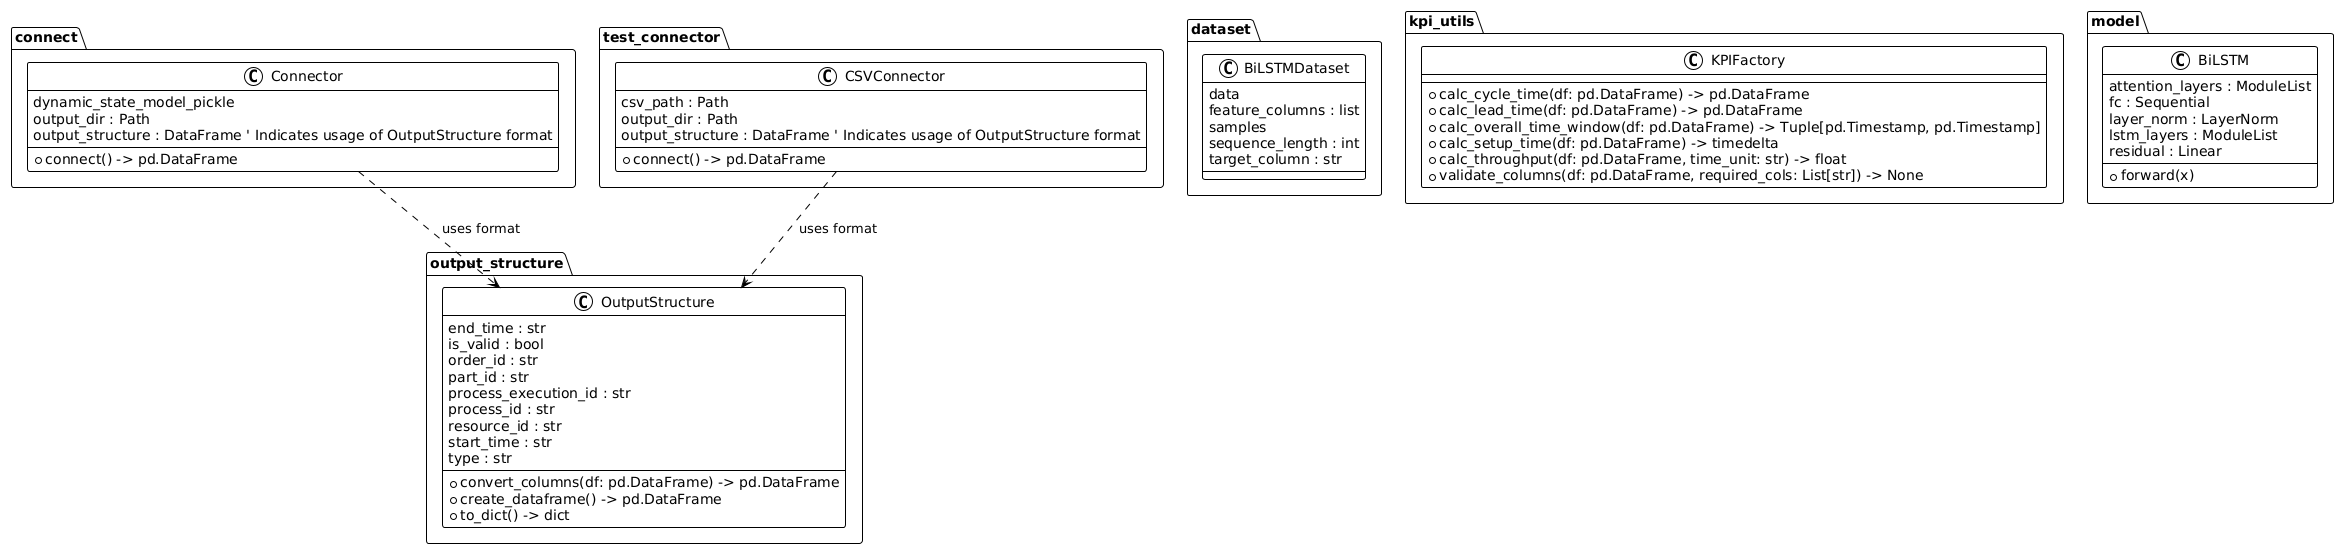
\includegraphics[width=1\textwidth]{figures/code.png}
  \caption[UML Diagram of the Implementation]{Unified Modelling Language (\gls{uml}) diagram of the ResNet-\gls{bilstm}-Attention framework for validating \gls{sbdt} in manufacturing environments.}
  \caption*{Source: Author's illustration.}
  \label{fig:uml-diagram}
\end{figure}

The \gls{uml} model \autocite{PlantUML} in \autoref{fig:uml-diagram} illustrates the systems architecture, which consists of several components that interact to achieve the validation of \gls{sbdt}. The components include:
\begin{itemize}
  \item \textbf{Data Connectors:} In the given code, two classes \texttt{InputStructure} and \texttt{OutputStructure} are responsible for reading and writing data. The \texttt{InputStructure} class reads raw data from the twin simulation, while the \texttt{OutputStructure} class writes the processed data into the \gls{ocel} format developed for this framework, see \autoref{sec:event_log_processing}. The connector assigns IDs by enumeration for different parts, resources, and processes. The IDs are used to identify the different components in the manufacturing process. This is a requirement for \gls{oced}. The mapping is returned as \gls{json} files for each category, respectively.
  \item \textbf{KPIFactory:} Contains utility functions to calculate a diverse set of \gls{kpi}s for \gls{ppc} evaluation of the process.
  \item \textbf{Baseline Model:} Implements a baseline model for comparison with the ResNet-\gls{bilstm}-Attention model. This model serves as a reference point to evaluate the performance of the more complex architecture.
  \item \textbf{PyTorch DataSet and DataLoader:} Handles the conversion of raw data into a format suitable for the ResNet-\gls{bilstm}-Attention model.
  \item \textbf{ResNet-\gls{bilstm}-Attention:} The core model that combines ResNet and \gls{bilstm} architectures with attention mechanisms to learn from the data.
\end{itemize}

\subsection{Tech Stack and Setup}
The implementation is built with Python 3.12 \autocite{Python}, using the following frameworks and libraries:

\begin{itemize}
  \item \textbf{PyTorch:} Powers the deep learning components, chosen for its dynamic computational graph that supports complex architecture development and debugging \autocite{PyTorch}.
  \item \textbf{Pandas \& NumPy:} Handle data manipulation, transformation, and numerical operations \autocite{NumPy, Pandas}.
  \item \textbf{Scikit-Learn:} Provides implementation of the baseline model and evaluation metrics \autocite{Scikit-Learn}.
  \item \textbf{Matplotlib \& Graphviz:} Generate visualizations of model architecture and performance \autocite{Matplotlib, Graphviz}.
  \item \textbf{UV Package Manager:} Ensures reproducible dependency management with exact version pinning \autocite{UV}.
\end{itemize}

PyTorch was preferred over TensorFlow due to its flexibility and ease of use, especially for research purposes. The implementation is designed to be modular and extensible, allowing for future enhancements and adaptations to different manufacturing environments.
The system is designed to run on a standard workstation with a multi-core \gls{cpu} and an optional \gls{gpu} for accelerated training. The given framework utilizes \gls{cuda} \autocite{NVIDIA_CUDA} for \gls{gpu} acceleration.

\section*{Data Preprocessing}
\label{sec:event_log_processing}

After laying out the architecture and system setup, this section focuses on the data preprocessing steps necessary for preparing the input data for the baseline model.

\subsection{OCEL Format}

Both models used in this thesis require the input data to be in the \gls{ocel} format, see \autoref{sec:object-centric-event-logs}. The columns are inspired by the \gls{sbdt} comparison model by \textcite{Schwede2024}. For the given framework, the format is expected as input in the following format:

\begin{table}[htbp]
  \centering
  \caption[Illustrative Manufacturing OCEL]{Detailed structure, data types, and description of the processed manufacturing \gls{ocel}.}
  \label{tab:output-structure-detailed}
  \begin{tabular}{l l p{6cm}} % l=left-aligned, p{width}=paragraph column
    \toprule
    \textbf{Column Name}            & \textbf{Data Type}       & \textbf{Description}                                                                                             \\
    \midrule
    \texttt{process\_execution\_id} & \texttt{int}             & Unique identifier for the specific process recorded.                                                             \\
    \texttt{order\_id}              & \texttt{Index (int/str)} & Identifier for the overall manufacturing order this event belongs to.                                            \\
    \texttt{start\_time}            & \texttt{Timestamp [UTC]} & The precise timestamp marking the beginning of the event, adjusted to UTC.                                       \\
    \texttt{end\_time}              & \texttt{Timestamp [UTC]} & The precise timestamp marking the end of the event, adjusted to UTC.                                             \\
    \texttt{duration}               & \texttt{float} (seconds) & The calculated duration of the event (\texttt{end\_time} - \texttt{start\_time}) in total seconds.               \\
    \texttt{part\_id}               & \texttt{int}             & Identifier for the specific part or component being processed or handled during the event.                       \\
    \texttt{resource\_id}           & \texttt{int}             & Identifier for the machine, station, or other resource involved in the event.                                    \\
    \texttt{process\_id}            & \texttt{int}             & Identifier indicating the type of process step or operation performed (e.g., milling, assembly).                 \\
    \texttt{type}                   & \texttt{str}             & A textual description or category classifying the type of data recorded.                                         \\
    \texttt{is\_valid}              & \texttt{bool}            & Boolean flag indicating whether the recorded event sequence or outcome is considered valid in the given setting. \\
    \bottomrule
  \end{tabular}
  \caption*{Source: Authors tabulation.}
\end{table}

The terms are consistent with the upper cited framework. For the model components, following features may be considered, here already enriched by feature enginnering performed in \autoref{sec:feature-engineering}:

\begin{enumerate}
  \item \textbf{Time Model:} \texttt{duration}, \texttt{sequence\_number}, \texttt{hour\_of\_day\_cos}, \texttt{hour\_of\_day\_sin}, \texttt{day\_of\_week\_cos}, \texttt{day\_of\_week\_sin}, \texttt{is\_break}, \texttt{is\_not\_weekday}.

  \item \textbf{Transition Model:} \texttt{part\_id}, \texttt{resource\_id}, \texttt{sequence\_number}, \texttt{duration}.

  \item \textbf{Transformation Model:} \texttt{part\_id}, \texttt{process\_id}, \texttt{sequence\_number}.

  \item \textbf{Quality Model:} Exclusion of quality information in the given model.

  \item \textbf{Resource Model:} \texttt{resource\_id}, \texttt{part\_id}, \texttt{process\_id}.

  \item \textbf{Resource Capacity Model:} \texttt{resource\_id}; Note: Insufficient data available for detailed capacity modelling.

  \item \textbf{Process Model:} \texttt{process\_id}, \texttt{duration}, \texttt{sequence\_number}.

  \item \textbf{\gls{kpi}-based Features:} \texttt{throughput}, \texttt{cycle\_time\_sec}, \texttt{lead\_time\_sec}, \texttt{setup\_time\_sec}.
\end{enumerate}

This table does not forbid adding relational logic by the modeller. For example, each \gls{id} may be a foreign key to another table. Each row in the \gls{ocel} represents a single event instance. This schema aligns with \gls{oced} principles (\autoref{sec:object-centric-event-logs}) by explicitly linking each recorded event instance (\texttt{process\_execution\_id} per timestamp) to the multiple object instances (\texttt{order\_id}, \texttt{part\_id}, \texttt{resource\_id}, \texttt{process\_id}) involved in its execution. This inherent multi-object relationship within each event record is important for modelling complex process dependencies. The structure empowers the representation of complex control flows often found in manufacturing. Parallel execution paths (AND-split $\wedge$)\footnote{The AND-split pattern means concurrent execution paths within a process, where multiple activities can be executed simultaneously. Here, this can be the case when different parts are prepared for further manufacturing in parallel because they dont depend on each other.} can be inferred by identifying events associated with different resources or process steps occurring \textit{within} overlapping time intervals (\texttt{start\_time}, \texttt{end\_time}) but related to shared object instances, such as a common \texttt{order\_id}. Alternative paths and process variants (exclusive OR-split $\oplus$)\footnote{The XOR split means mutually exclusive execution paths, where exactly one path is chosen from multiple alternatives. For the given \gls{dmfs}, different product configurations may be produced by performing mutually exclusive process steps.} are explicitly captured through the diversity of event sequences observed across different process instantiations, for example grouped by \texttt{order\_id}. The log records exactly which path or sequence of activities occurred for each instance. The object-centric nature enriches this analysis by providing context that can explain why a particular variant or choice was executed. The \gls{ocel} retains its sequential linear character by grouping it by \texttt{order\_id} and sorting ascending related to \texttt{end\_time}. This allows for the reconstruction of the process flow. The use-case in \autoref{chap:case-study} will engineer further features from the \gls{ocel} format.

While conciseness of the data structure was a given requirement, the \gls{ocel} format is not fully compliant with the \gls{oced} standard \autocite{van2023object}. The \gls{ocel} format used in this thesis is rather simplified. Specifically, this simplification means the schema does not include distinct tables for object instances and their types, explicit modelling of static O2O relationships (\autoref{sec:object-centric-event-logs}) or the capability to store timestamped attributes associated directly with objects rather than events. Despite these omissions the implemented structure retains the core \gls{oced} principles. The goal is rather to \textit{learn} these relationships from the data itself.

\section{Model Implementation}

This section details the implementation of the models used for \gls{sbdt} validation. Two distinct approaches are used: An interpretable whitebox baseline model and the more complex ResNet-\gls{bilstm}-Attention blackbox model. The primary goal is to compare their ability to classify process executions as `valid' or `invalid' based on the \gls{ocel} data.

The core modelling task is binary classification using the \texttt{is\_valid} column as the target variable. This classification is a key component within the broader \gls{vvuq} process. While the models predict validity, \gls{uq} is addressed through statistical methods like permutation testing (\autoref{sec:permtest}). Verification often requires subsequent manual analysis by the modeller when invalidity is detected\footnote{While manual verification is necessary upon detecting invalidity, the framework aims to automate the continuous monitoring process, saving significant effort when the system operates as expected.}. The whitebox model, specifically a Decision Tree Classifier (\texttt{DecisionTreeClassifier} from Scikit-Learn \autocite{Scikit-Learn}), provides an interpretable baseline. Its transparency allows for direct rule extraction and can help in diagnosing issues like data leakage or verifying if specific model components (like time- or resource model) are adequately represented and learned from the data, complementing techniques like \gls{afs} and sanity checks (\autoref{sec:sanity-check}, \textcite{adebayo2018sanity}).

The blackbox model, the ResNet-\gls{bilstm}-Attention network (\autoref{sec:integrated_architecture}), prioritizes capturing complex sequential patterns, potentially achieving higher predictive performance at the cost of direct interpretability. Both models are trained and evaluated on the same dataset, processed as described below, using identical metrics (\autoref{sec:metrics-theory}) for fair comparison, with results presented in \autoref{chap:case-study}.

To enable the whitebox model to capture some sequential context and ensure fair comparison, the data is grouped by \texttt{order\_id} and sorted chronologically by \texttt{end\_time}. However, model limitations remain, as \gls{dtree}s are not naturally suited for sequence learning, unlike the ResNet-\gls{bilstm}-Attention architecture. For the train-test split, a random split strategy is employed. Despite the sequential nature of the data, random splitting is chosen over a temporal split to mitigate potential temporal bias arising from potentially incomplete process traces at the split point, following insights from \textcite{morita2022investigation}.

\subsection{Whitebox Baseline Model}
A Decision Tree Classifier (\texttt{sklearn.tree.DecisionTreeClassifier} \autocite{Scikit-Learn}) serves as the interpretable whitebox baseline. Its primary function is to provide a performance reference point against the more complex blackbox model and to offer insights into feature importance and potential data issues due to its transparent nature.

\subsection{ResNet BiLSTM Multi-Head Self-Attention Network}
The primary model implemented is the ResNet-\gls{bilstm}-Attention network (\autoref{sec:integrated_architecture}), designed to capture temporal dependencies within the manufacturing process data. This model leverages the PyTorch framework \autocite{PyTorch}. Data ingestion is managed by custom \texttt{DataSet} and \texttt{DataLoader} classes, which prepare the \gls{ocel} data into sequences suitable for the network and handle batching and shuffling during training.

\begin{figure}[htbp]
  \centering
  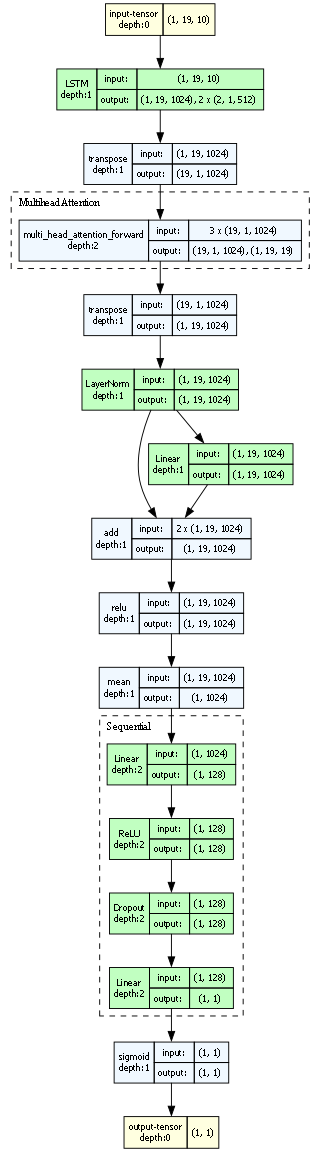
\includegraphics[width=0.4\textwidth]{figures/architecture.png}
  \caption[ResNet-BiLSTM-Attention Architecture]{ResNet-\gls{bilstm}-Attention architecture. Several layers are stacked, including \gls{bilstm}, residual connections, and attention mechanisms. The model processes input sequences, applies self-attention, and outputs a single value for binary classification.}
  \label{fig:architecture}
  \caption*{Source: Author's Torchview illustration.}
\end{figure}

The network architecture, visualized in \autoref{fig:architecture}, integrates Bidirectional Long Short-Term Memory (\gls{bilstm}) layers with Multi-Head Self-Attention and Residual Connections using \texttt{torch.nn} modules. The key components are:

\begin{enumerate}
  \item \textbf{Input/Configuration:} Initialized with hyperparameters: \texttt{input\_size} ($D$, number of features), \texttt{hidden\_size} ($H$, \gls{lstm} state dimensionality), \texttt{num\_layers} ($N$, number of stacked \gls{lstm}/Attention blocks), and \texttt{attention\_heads} ($A$, number of attention heads).

  \item \textbf{\gls{bilstm} Layers:} $N$ stacked \texttt{nn.LSTM} layers (\texttt{bidirectional=True}) process sequences bidirectionally. Each layer outputs a $2H$-dimensional representation per time step. Dropout is applied between layers.

  \item \textbf{Multi-Head Self-Attention:} An \texttt{nn.MultiheadAttention} layer follows each \gls{bilstm} layer, allowing the model to weigh the importance of different time steps within the sequence relative to each other.

  \item \textbf{Layer Normalization \& Residual Connections:} \texttt{nn.LayerNorm} stabilizes activations post-attention. A residual connection adds the block's input to its normalized output, followed by \texttt{\gls{relu}} activation, aiding gradient flow.

  \item \textbf{Sequence Pooling:} Temporal mean pooling (\texttt{torch.mean}) aggregates the final block's sequence output ($Batch \times Sequence Length \times 2H$) into a fixed-size vector ($Batch \times 2H$).

  \item \textbf{Final Classifier:} A feed-forward network (\texttt{nn.Sequential}), typically with linear layers, \texttt{ReLU}, and Dropout, maps the pooled representation to a single output logit.

  \item \textbf{Output Activation:} \texttt{torch.sigmoid} converts the logit to a probability $[0, 1]$ for binary classification. A threshold $\tau = 0.9$ is used during evaluation.

  \item \textbf{Weight Initialization:} Linear layers use Kaiming Normal initialization.
\end{enumerate}

For training (\texttt{model.train()}), the \textit{\gls{adam}} optimizer (\autoref{eq:adam}, \autocite{kingma2014adam}) is used with an initial learning rate of $0.001$ and Binary Cross-Entropy loss (\texttt{nn.BCELoss}, \autoref{eq:bce}). Input sequences have a length of $19$.\footnote{The sequence length was determined through hyperparameter tuning as optimal for the given dataset. This often corresponds to typical trace lengths.} Dropout ($p=0.3$) is applied in the \gls{bilstm} layer and the final classifier for regularization. The architecture uses $N=1$ \gls{bilstm} layer with $H=512$ hidden units per direction, followed by $A=4$ attention heads. The classifier head has an intermediate dense layer of $128$ units. Theoretical foundations are in \autoref{sec:lstm} onwards.

A \textit{ReduceLROnPlateau} scheduler (\texttt{torch.optim.lr\_scheduler.ReduceLROnPlateau}) adjusts the learning rate, decreasing it by a factor of $0.1$ if training loss plateaus for $5$ epochs (\texttt{patience=5}), although rapid convergence in initial tests made this less critical.\footnote{While implemented for robustness, the scheduler's effect was minimal in initial experiments due to quick convergence.} Training runs for $10$ epochs (\texttt{num\_epochs=10}) with shuffled mini-batches of size $32$ (\texttt{batch\_size=32}). Each epoch includes forward/backward passes and optimizer steps, with loss tracked for monitoring.

\section{Model Evaluation}

Evaluation follows the principles from \autoref{sec:metrics-theory}. The model is set to evaluation mode (\texttt{model.eval()}) to disable dropout and fix \texttt{BatchNorm} statistics, ensuring deterministic output. Gradients are then disabled (\texttt{torch.no\_grad()}) for efficiency. The test set is processed batch-wise to generate predictions.

Performance is assessed using the \texttt{evaluate\_model()} method, which uses \texttt{sklearn.metrics} to compute a classification report, confusion matrix (\autoref{tab:confusionmatrix}), accuracy (\autoref{eq:accuracy}), precision (\autoref{eq:precision}), recall (\autoref{eq:recall}), F1-score (\autoref{eq:F1-score}), and the \gls{roc} \gls{auc} score (\autoref{eq:auc}). These metrics facilitate comparison between the baseline and ResNet-\gls{bilstm}-Attention models, evaluate performance on the holdout set, and help in diagnosing issues, potentially informed by \gls{afs} results.

A classification threshold of $\tau = 0.9$ is applied to the model's output probabilities to categorize instances as `valid' ($p \geq 0.9$) or `invalid' ($p < 0.9$). This value, higher than the typical $0.5$, reflects a lower tolerance for \gls{fp} (mistaking simulated/invalid data for real/valid data) in the manufacturing validation context, a common practice in anomaly detection scenarios where the cost of such errors is high.

It is crucial to distinguish this operational classification threshold $\tau$ from the rejection rate ($RR$) used in permutation testing (\autoref{sec:permtest}, \autoref{sec:model-logic}). The threshold $\tau=0.9$ is a specific decision boundary used post-training to classify individual instances, directly impacting metrics like precision and recall calculated at this single operating point. Conversely, the permutation test evaluates the overall statistical significance of the model's ability to discriminate between the real and simulated data distributions, typically using the \gls{roc} \gls{auc} score which considers performance across \textit{all} possible thresholds. The resulting $RR$ quantifies the consistency of this significant discriminative ability across multiple test runs. Therefore, a high $RR$ indicates robust differentiation capability, independent of the specific operational threshold $\tau$ chosen based on application-specific risk tolerance.